\section{Problemstellung} \label{sec:Problemstellung}
Die fundamentale und schwerste Frage, bei den Stadt-Analogien ist, wie das Layout der Stadt aussehen soll.




\subsection{Das Treemap Problem} \label{sec:TreemapProblem}
In Abschnnit \ref{sec:Treemap} wurde aufgezeigt, dass bereits der initiale Algorithmus von Johnson und Shneiderman \cite{johnson1991tree} ein fundamentales Problem aufweist, wenn Treemaps mit Abständen zwischen Knoten dargestellt werden sollen. 
\begin{itemize}
    \item Da der Abstand von der Fläche der Knoten abgezogen wird, ist die dargestellte Fläche nicht mehr proportional zum Wert des Knotens.
    \item Durch das Abziehen der Abstände kann es passieren, dass Knoten verschwinden, wenn entweder die Länge oder die Breite der Knoten kleiner oder gleich dem Abstand ist.
\end{itemize}

In den Abbildungen \ref{fig:zeroMarginArtificialMap}, \ref{fig:fiveMarginArtificialMap} und \ref{fig:tenMarginArtificialMap} sind Treemap Layouts abgebildet, die mit dem Squarify Algorithmus nach Abschnitt \ref{sec:Squarify} generiert wurden. Der Visualierten Metriken sind händisch erstellt, um das Problem zu verdeutlichen (siehe Anhang HIER REF EINRÜGEN). In Bild \ref{fig:zeroMarginArtificialMap} sind alle Knoten sichtbar und die Fläche der Knoten ist proportional zu den Werten der Knoten. In Bild \ref{fig:fiveMarginArtificialMap} sind immernoch alle Knoten sichtbar, aber die Fläche der Knoten ist nicht mehr proportional zu den Werten der Knoten. Zum Beispiel hat der Große Knoten mit Wert 3000 eine Fläche von ca. 2600, wärend der kleine Knoten oben links mit Wert 30 nur eine Fläche von ca. 5 hat. In Bild \ref{fig:tenMarginArtificialMap} mit Abstand 10 sind dann schon einige Knoten (zum beispiel der Eben genannte knoten oben links) nicht mehr sichtbar, da die breite der Knoten kleiner als der Abstand ist. 

\begin{figure}
    \centering
    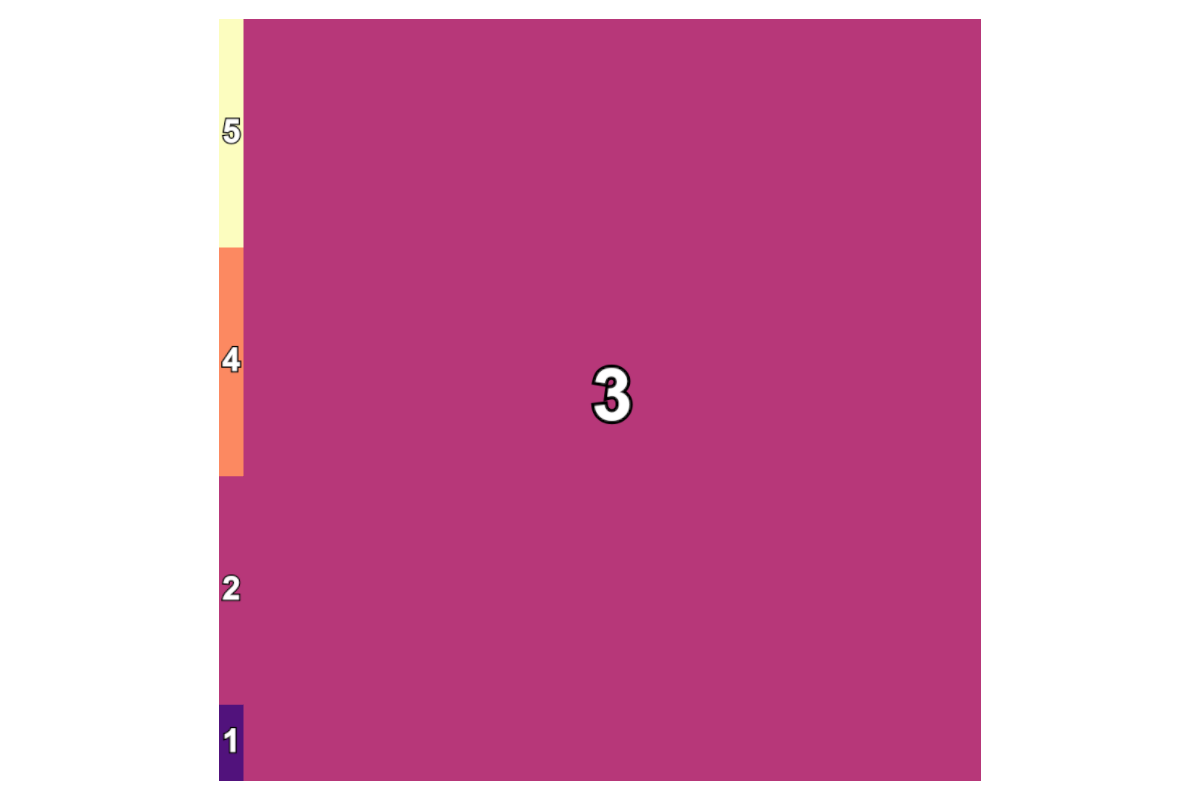
\includegraphics[width=0.8\textwidth]{images/zeroMarginArtificialMap.png}
    \caption{Treemap Layout generiert mit dem Squarify Algorithmus nach Abschnitt \ref{sec:Squarify} mit einem Abstand von 0} 
    \label{fig:zeroMarginArtificialMap}
\end{figure}

\begin{figure}
    \centering
    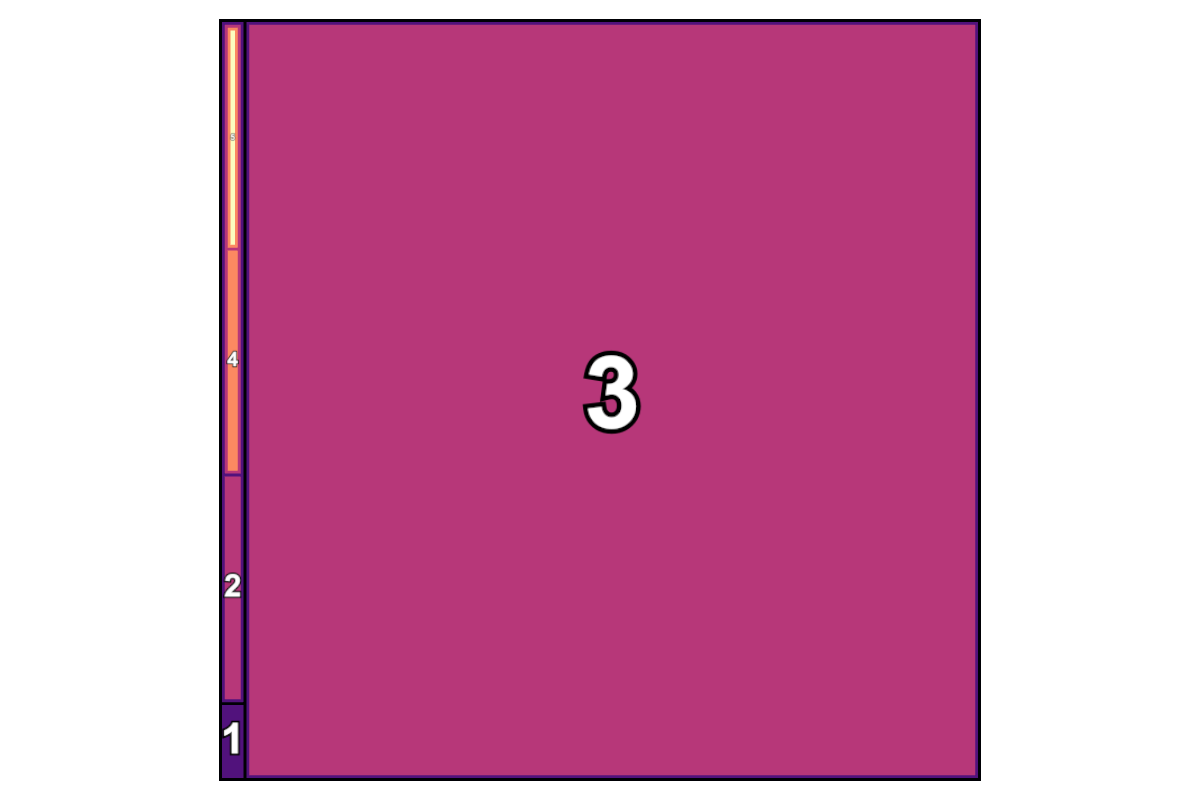
\includegraphics[width=0.8\textwidth]{images/fiveMarginArtifialMap.png}
    \caption{Treemap Layout generiert mit dem Squarify Algorithmus nach Abschnitt \ref{sec:Squarify} mit einem Abstand von 5} 
    \label{fig:fiveMarginArtificialMap}
\end{figure}

\begin{figure}
    \centering
    
\includegraphics[width=0.8\textwidth]{images/tenMarginArtifialMap.png}
    \caption{Treemap Layout generiert mit dem Squarify Algorithmus nach Abschnitt \ref{sec:Squarify} mit einem Abstand von 10} 
    \label{fig:tenMarginArtificialMap}
\end{figure}

Es ist nicht trivial dieses Problem zu lösen, da es die grundlegende Annahme der Treemap Algorithmen verletzt, dass die Fläche aller Knoten bekannt ist, bevor die Knoten plaziert werden. 
Bevor die Knoten plaziert werden, ist nicht klar, wie die Fläche der Knoten aussieht, das heißt, es ist auch nicht klar, wie viel Platz für die Abstände zwischen den Knoten benötigt wird. Dies wird klar wenn man sich die Abbildung \ref{fig:marginAreaDifference} anschaut. Dort sieht man, dass die Fläche, die für Knoten in ihren Eltern benötigt wird, größer ist als die Fläche, die für die Knoten selbst benötigt wird und diese benötigte Fläche stark vom Layout der Knoten selbst abhängt. Somit ist auch unklar, wie groß die Fläche aller elternknoten sind. 

\begin{figure}
    \centering
    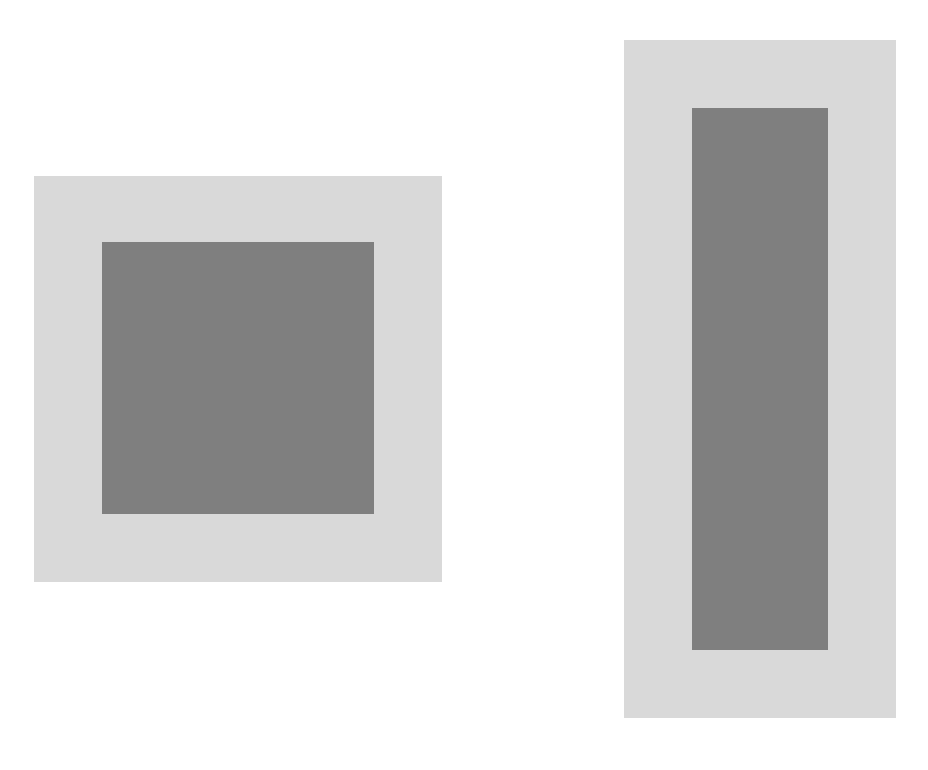
\includegraphics[width=0.8\textwidth]{images/marginArea.png}
    \caption{Abbildung eines zweier Rechecke mit der Fläche 16 in dunkel grau und in hellgrau der Abstand von 1 um die Flächen herum. Das Linke Rechteck (4x4) mit Abstand nimmt eine Fläche von 25 (5x5) ein. Das rechte Rechteck (2x8) mit Abstand nimmt eine Fläche von 40 (4x10) ein.}
    \label{fig:marginAreaDifference}
\end{figure}

Das Problem ist jetzt aber, dass wenn die Fläche der Knoten nicht bekannt ist auch das Layout der Knoten nicht berechnet werden kann, da die Fläche der Knoten für das Layout benötigt wird. Hier ergibt sich also ein Zirkelschluss: Die Fläche ist nicht klar, ohne das Layout und das Layout kann nicht berechnet werden, ohne die Fläche zu kennen.
